\documentclass[a4paper, twoside, 12pt,french]{report}

\usepackage[utf8]{inputenc}
\usepackage[T1]{fontenc}
\usepackage[francais]{babel}
\usepackage{lmodern}
\usepackage[top=2.5cm, bottom=2.5cm, left=2.5cm, right=2.5cm]{geometry}
\usepackage{graphicx}
\usepackage{cite}
\usepackage[nottoc,notlot,notlof]{tocbibind} % Ajoute la bibliographie dans la table des matières (toc)
\usepackage{fancyhdr} % Hauts de page
\usepackage{hyperref} % Liens
\usepackage{listings} % Code

%%%%% Header %%%%%
\fancyhead[RO,LE]{\thepage}
\fancyhead[LO]{\itshape\nouppercase{\leftmark}}
\fancyhead[RE]{\itshape\nouppercase{\rightmark}}
\fancyfoot{}

%\renewcommand{\headrulewidth}{0pt} % Epaisseur de la ligne sous le header
\geometry{headheight=16pt} % Nécessaire pour fancyhdr
%\setlength{\headheight}{16pt} % Nécessaire pour fancyhdr

\raggedbottom % Evite que la page couvre tout l'espace vertical avec des espaces

%%%%% Code %%%%%
\lstset{
breaklines=true,
numbers=left,
numbersep=10pt,
frame=lrtb
}

\begin{document}

\begin{titlepage}
\center

\textsc{\LARGE Université catholique de Louvain}\\[1cm]
\textsc{\Large Travail de fin d'études}\\[2cm]


\includegraphics[scale=.15]{UCL_mention_pantone282.jpg}\\[1.5cm]

% Titre
\textsc{\Large }\\[1.5cm]

\begin{minipage}{0.4\textwidth}
\begin{center}
%\large \emph{Auteur :} \\
\large Antoine \textsc{Marchal}
\end{center}
\end{minipage}\\[3.5cm]

\begin{minipage}{0.4\textwidth}
\begin{flushleft} \large
\emph{Promoteurs :} \\
Olivier \textsc{Bonaventure}\\
Pierre \textsc{Reinbold}
\end{flushleft}
\end{minipage}
~
\begin{minipage}{0.4\textwidth}
\begin{flushright} \large
\emph{Lecteurs :} \\
 \textsc{}\\
 \textsc{}
\end{flushright}
\end{minipage}\\[1.5cm]


{\normalsize Mémoire réalisé en vue de l'obtention du grade de\\
\emph{Master [120] en Sciences Informatiques} (option \emph{Networking \& Security})}\\[1.5cm]

{\huge Version temporaire, compilée le \today}
%{\normalsize Louvain-la-Neuve, Belgique}\\
%{\normalsize Année académique 2013-2014}

\end{titlepage}

%%% Table des matières
\addtocontents{toc}{\protect\thispagestyle{empty}} % Enlève le numéro de page sur la première page du toc
\pagestyle{empty} % Enlève le numéro de page sur les autres pages du toc
\newgeometry{top=1.5cm, bottom=2cm, left=2.5cm, right=2.5cm}
\tableofcontents
\restoregeometry
\clearpage % Nécessaire pour ne pas avoir fancyhdr sur la dernière page du toc
%%%
\pagestyle{fancy}
\chapter{Introduction}
\section{Motivation et problématique}
Notre navigation sur Internet est de plus en plus scrutée par diverses organisations, que ce soient des entreprises commerciales ou des agences gouvernementales. D'ailleurs, des révélations récentes \cite{WikipediaFR_RES} ont permis de mettre en lumière un système élaboré destiné à surveiller les utilisateurs d'Internet.

Ce travail se focalise sur la surveillance opérée par les entreprises commerciales. En effet, elles essaient de nous suivre à la trace afin de déterminer nos habitudes et nos préférences. Avec l'aide de ces précieuses informations, elles peuvent alors mieux cibler nos besoins et nous proposer des biens et des services qui sont censés nous intéresser davantage, voire anticiper nos intentions\cite{MD1}.

Cette pratique est de plus en plus répandue sur les sites de vente en ligne, grâce à l'historique de nos consultations et achats.

D'autres formes de surveillance plus vicieuses existent également. Imaginons que vous souhaitiez voyager vers un pays exotique et que vous consultez le prix des billets d'avion vers cette destination sur le site d'une compagnie aérienne. Lors d'une consultation ultérieure, le prix a augmenté et vous vous empressez alors d'acheter le billet craignant que son prix ne continue d'augmenter. Malheureusement pour vous, celui-ci a en fait été gonflé pour vous pousser à l'achat.

Les plus grosses régies publicitaires sont installées sur un grand nombre de sites et lors de chaque visite, elles enregistrent les traces que vous laissez. En regroupant toutes les informations disséminées sur ces différents sites, elles sont alors en mesure d'établir votre profil. Les détails de celui-ci peuvent se revendre à prix d'or auprès d'autres compagnies. Il est évidemment plus facile de cibler un segment constitué de personnes dont on connaît le profil socio-démographique, le sexe, l'âge, les intérêts,...

Avez-vous déjà remarqué que le contenu des publicités s'adaptait en fonction de vos requêtes effectuées sur les moteurs de recherche ou des sites que vous visitez ?

Comme vous pouvez le remarquer avec ces différents exemples de la vie quotidienne, la surveillance des utilisateurs d'Internet peut générer plusieurs inconvénients qui nous touchent directement. Il est donc intéressant d'analyser cette surveillance et déterminer par quels moyens elle s'opère. Afin de préserver notre vie privée sur Internet, il est nécessaire de connaître comment nous sommes identifiés. Il faut également s'assurer que les outils dont nous disposons afin de nous protéger soient réellement efficaces et adaptés à nos besoins.


%%%%%%%%%%%%%%%%%%%%%%%%%%%%%%
\section{La vie privée}
Le respect de la vie privée est intimement lié à l'évolution de la surveillance.
Il y a toujours eu des conflits entre les personnes qui estiment que tout le monde doit pouvoir utiliser et partager une technologie permettant de sécuriser ses communications et les gouvernements qui souhaiteraient garder la possibilité d'écouter ces communications. Prenons l'exemple du gouvernement américain qui avait peur de passer d'un monde où il avait un contrôle total à un monde où il n'en avait plus. En conséquence, il a considéré l'export de la cryptographie hors des USA équivalent à l'export de munitions. Ainsi, afin de dévoiler les sources de PGP (Pretty Good Privacy, un logiciel de chiffrement et de déchiffrement cryptographique) au monde entier, son auteur a usé d'une astuce en publiant un livre qui en contient le code source complet (l'export de livres est protégé par le Premier Amendement) \cite{youtube_moxie_marlinspike}.
\newline

Les programmes de surveillance du passé peuvent être considérés comme de la "surveillance de proximité", où un gouvernement tentait d'utiliser la technologie afin de surveiller les communications lui-même. Les programmes actuels marquent une transition vers la "surveillance oblique" dans laquelle un gouvernement va plus souvent se rendre aux endroits où les informations sont accumulées (fournisseurs d'adresses e-mail, moteurs de recherche, réseaux sociaux et télécoms) \cite{wired_nothing_to_hide}.
\newline

En 2001, John Poindexter a voulu mettre en place le programme \textit{Total Information Awareness} qui consistait en un système de data mining. Celui-ci devait enregistrer tous les e-mails, tout le trafic web, tout l'historique des cartes de crédit et tous les dossiers médicaux. Le but était ensuite de développer une technologie afin d'extraire les données dont on avait besoin. Lors de sa conférence à la DEF CON 18, Moxie Marlinspike a d'ailleurs tourné en ridicule le logo du programme (\autoref{IAO_logo}) en expliquant qu'il était déconseillé d'utiliser un logo qui inspirait plutôt la peur. D'ailleurs, le projet a été annulé car il a reçu beaucoup de contestations. Cependant, lorsque l'on regarde ce que Google fait aujourd'hui, c'est exactement la même chose, voire pire. Or, personne ne proteste et de surcroît, tout le monde utilise ses services !
\begin{itemize}
  \item Les emails sont enregistrés par Gmail.
  \item Le trafic web est enregistré par Google Analytics.
  \item L'historique des cartes de crédit est enregistré par Google Checkout.
  \item Les dossiers médicaux sont enregistrés par Google Health.
  \item L'historique des positions GPS est enregistré par Android.
  \item ...
  %\newline
\end{itemize}
De plus, on sait que Google a la capacité d'extraire de manière efficace les informations qu'il désire afin de les monétiser avec des publicités. Lorsque le CEO de Google, Eric Schmidt, déclare : "If you have something that you don't want anyone to know, maybe you shouldn't be doing it in the first place" \cite{privacy_eric_schmidt}, cela fait froid dans le dos.

\begin{figure}[h]
	\centering
	
\includegraphics[scale=0.2]{figures/IAO-logo.png}
	\caption{\label{IAO_logo}Le logo officiel du programme \textit{Total Information Awareness}}.
\end{figure}

Dans sa conférence, Moxie Marlinspike utilise un autre exemple : personne n'accepterait de porter un trackeur monitoré par l'Etat mais tout le monde possède et porte un GSM en permanence. Or, celui-ci envoie en temps réel sa position à l'opérateur qui est obligé de délivrer cette information si on la lui demande. Pour lui, il y a cependant une différence essentielle : le choix. Nous choisissons de posséder un GSM afin de communiquer mais nous refuserions un dispositif de traçage s'il nous était imposé.
\newline

%%%%%

Maintenant, passons au sujet de la vie privée.\\
D'après Moglen \cite{Moglen_part2}, le concept de vie privée englobe 3 éléments.
\begin{itemize}
  \item La confidentialité : la capacité de garder des messages privés c'est-à-dire que leur contenu n'est connu que de ceux à qui ils sont destinés.
  \item L'anonymat : la capacité d'envoyer des messages sans savoir de qui ils proviennent ni à qui ils sont destinés, même si leur contenu est ouvert.
  \item L'indépendance : la capacité de prendre des décisions librement, sans que la confidentialité ou l'anonymat ne soient violés.
\end{itemize}

Pour lui, si l'un de ces éléments n'est pas respecté, on ne peut pas avoir de gouvernement démocratique car la vie privée en est une condition nécessaire.
\newline

Il explique également qu'on ne devrait pas voir la vie privée comme une transaction. En effet, ceux qui veulent profiter de nos informations souhaitent définir la vie privée comme un concept que l'on peut négocier. Ainsi, ils nous offrent un service gratuit comme l'accès à une messagerie mais en échange, ils lisent nos mails. Pour eux, il s'agirait seulement d'une transaction entre deux parties. Cependant, si on y réflechit, ce n'est pas une transaction quelconque car tout ceux qui nous écrivent sont aussi impliqués dans cet accord, qui était supposé être bilatéral.

Rien n'est gratuit dans la vie et cela l'est également sur Internet. En réalite, le prix à payer est de dévoiler des informations personnelles qui peuvent potentiellement être exploitées afin de rapporter de l'argent.
\newline

Les exemples de l'introduction montrent déjà clairement que la surveillance des sites web peut nous coûter de l'argent en nous incitant à consommer plus. Mais les risques de cette surveillance peuvent aller bien au-delà. En effet, la liste des sites web visités par une personne peut en révéler beaucoup sur sa situation familiale, financière ou sanitaire.
\newline

Imaginons une situation où le directeur des ressources humaines d'une entreprise reçoit des CV. Il décide de trouver davantage d'informations au sujet des candidats et pour cela, tape leur nom dans un moteur de recherche. Il pourrait tomber sur la photo d'une jeune femme portant un bébé dans ses bras ou sur la photo d'une jeune femme seule. Pensez-vous qu'elles aient la même chance d'être rappelées pour un entretien ?

Lors d'une expérience menée avec son équipe, Alessandro Acquisti a créé des profils Facebook en modifiant certaines de leurs caractéristiques. Il a ensuite envoyé des candidatures à différentes entreprises américaines et a analysé leur comportement face aux profils associés aux candidatures. Les résultats de l'expérience ont montré que les entreprises agissaient en fonction des informations qu'elles avaient trouvées sur les réseaux sociaux.
\newline

Face à la montée de la surveillance, certaines personnes affirment qu'elles n'ont rien à cacher.
La vie privée n'a rien à voir avec le fait d'avoir quelque chose de négatif à cacher \cite{TED_Alessandro_Acquisti}.
Nous faisons énormément de choses en privé qui ne sont pas considérées comme illégales mais que nous préférons garder pour nous. Mettre des rideaux à ses fenêtres n'est pas criminel, cela traduit juste notre envie de garder notre intimité, vie privée.

Que diraient-elles si leur gouvernement, avec l'aide de toutes les informations qu'il possède grâce à la surveillance, décidait que leurs actions étaient suspectes et que des sanctions étaient appliquées arbitrairement ?
On peut également tenter de les raisonner par cette simple question : donneriez-vous votre adresse, numéro de téléphone, carte de crédit et autres données personnelles à un inconnu dans la rue ?

%%%%%%%%%%%%%%%%%%%%%%%%%%%%%%
\section{Méthodologie utilisée}
Afin de répondre à la problématique de la surveillance sur Internet, il faut tout d'abord comprendre comment Internet fonctionne et en particulier, certains de ses mécanismes tels que les cookies.

Ensuite, il faut identifier la manière dont ces mécanismes peuvent être utilisés ou détournés afin de permettre le traçage des utilisateurs.

Grâce à ces connaissances, nous serons en mesure de détecter quels sont les moyens effectivement utilisés par les sites qui pratiquent cette surveillance et d'estimer son étendue sur un panel constitué des principaux sites web (classement Alexa \cite{AlexaTop}).

Pour terminer, nous pourrons déterminer si les outils censés protéger notre vie privée sont réellement efficaces. % et par quels moyens nous pourrions les améliorer.


\chapter{Protocoles et mécanismes d'Internet}

\section{Présentation du protocole HTTP}
HTTP (HyperText Transport Protocol) \cite{Obo_CNP3} est un protocole qui fournit les fondations du World Wide Web, il repose sur le modèle client-serveur dans lequel le client envoie une requête et le serveur retourne une réponse. Il est décrit par la RFC 2616 \cite{IETF_RFC2616}.
\newline

Les requêtes HTTP se composent de trois parties :
\begin{enumerate}
	\item Une ligne de requête (qui contient notamment une URI)
	\item Des entêtes (qui contiennent des paramètres pour la requête)
	\item Le corps de la requête (optionnel)
	\newline
\end{enumerate}

Lorsqu'un utilisateur clique sur un lien hypertexte via son navigateur, celui-ci se connecte à un serveur identifié par l'URI "Uniform Resource Identifier" présente dans ce lien. Le navigateur envoie alors une requête à laquelle le serveur répond puis le navigateur se déconnecte du serveur. L'on considère que la requête est sans état car à chaque fois que le navigateur crée une connexion pour une requête, le serveur la traite comme si c'était la première ; les requêtes sont donc indépendantes.
\newline

Les réponses HTTP se composent également de trois parties :
\begin{enumerate}
	\item Une ligne de statut (qui indique si la requête est réussie ou pas)
	\item Des entêtes (qui contiennent des informations sur la réponse)
	\item Le corps de la réponse
	\newline
\end{enumerate}

Il fallait trouver une solution afin d'avoir la possibilité de garder une certaine quantité d'informations entre des requêtes successives. Une première solution était de forcer l'authentification du client (comme pour FTP), cependant ce n'est pas toujours nécessaire ou applicable sur tous les sites web. Une seconde solution était d'utiliser les différents types d'entêtes \emph{Accept-*}, mais cela fournit des possibilités assez limitées. Une autre solution, qui est la plus largement adoptée, est l'utilisation d'un cookie HTTP.
\newline

Des exemples de requête et réponse HTTP sont disponibles dans la \autoref{http_request_example}.


%%%%%%%%%%%%%%%%%%%%%%%%%%%%%%
\section{Cookies}
La première description sur les cookies a été publiée sur le site web de Netscape Communications mais cette description était informelle. Le processus de standardisation des cookies a commencé en avril 1995 sur la liste de diffusion [www-talk], ensuite, l'IETF (Internet Engineering Task Force) a entrepris d'écrire un standard pour les cookies \cite{Kristol:2001:HCS:502152.502153}. C'est ainsi que la première RFC (RFC 2109) sur les cookies est parue en février 1997 \cite{IETF_RFC2109}, rendue obsolète en octobre 2000 par la RFC 2965 \cite{IETF_RFC2965}. Elle a également été remplacée, par la RFC 6265 en avril 2011 \cite{IETF_RFC6265}, qui est toujours d'application en ce jour et constitue la référence en ce qui concerne les cookies. Il est intéressant de noter qu'une section dédiée à la vie privée (section 7) est présente dans cette dernière RFC, ce qui constitue une nouveauté.
\newline

Un cookie est un petit fichier stocké en clair sur le disque dur de l'utilisateur par le navigateur. Il fait le lien entre la session de l'utilisateur et les données enregistrées par le site web (dans une base de données par exemple). Les cookies sont transmis dans les entêtes des requêtes et des réponses HTTP \cite{IETF_RFC6265}.
\newline

Dans sa réponse à une requête, un serveur peut envoyer des informations arbitraires (le cookie) dans un entête \textit{Set-Cookie}. Cette information peut contenir n'importe quoi et c'est elle qui permet au serveur de continuer là où il en était. Il peut s'agir d'un identifiant relatif à l'utilisateur, une clé dans une base de données,...
Le serveur peut ajouter des attributs afin de configurer les cookies (sections 5.2.1 à 5.2.6 de la RFC 6265) \cite{IETF_RFC6265} :

\begin{itemize}
	\item Expires et Max-Age : date d'expiration
	\item Domain : domaine
	\item Path : chemin
	\item Secure et HttpOnly : type de connexion
	\newline
\end{itemize}

Habituellement, le client est coopératif et renvoie l'information du cookie qui est stocké par le navigateur. Dans chaque requête ultérieure qu'il fait vers le serveur, le client indique cette information dans un entête \textit{Cookie}. Le serveur peut choisir de renvoyer un nouveau cookie dans ses réponses, ce qui remplacera automatiquement l'ancien cookie.
\newline

Il y a un contrat implicite entre le client et le serveur : ce dernier repose sur le client afin de sauvegarder son état et il espère qu'il lui sera retourné lors de la prochaine requête. Un cookie est donc une donnée que le serveur et le client se renvoient l'un et l'autre. La quantité d'informations est généralement petite et son contenu est à la discrétion du serveur. En effet, la plupart du temps, analyser le contenu du cookie ne révèle ni à quoi il est destiné ni la valeur qu'il représente.


%%%%%%%%%%%%%%%%%%%%%%%%%%%%%%
\section{Cache}
Dans le domaine informatique, un cache permet de garder une copie locale d'un élément afin de répondre rapidement à une requête. Au lieu de récupérer l'élément, le cache renvoie sa copie, ce qui permet de réduire sensiblement le temps de réponse.\\
Le principe de cache sur le protocole HTTP est défini dans la RFC 2616 \cite{IETF_RFC2616} (sections 13 et 14). Les mécanismes de cache peuvent être implémentés à différents niveaux :
\begin{itemize}
  \item sur le réseau qui délivre le contenu d'un site web (ex. : un CDN - "Content Delivery Network")
  \item sur l'application qui gère et affiche le contenu d'un site web (ex. : un CMS - "Content Management System")
  \item sur le serveur qui héberge le site web (ex. : Apache)
  \item via le navigateur Web du client qui stocke les fichiers sur le disque dur
  \newline
\end{itemize}

Lorsque que l'on navigue sur Internet, le cache du navigateur enregistre certaines ressources (images, feuilles de style, fichiers JavaScript, etc.) afin de ne pas devoir les recharger depuis le serveur lors des visites ultérieures. Par ailleurs, les administrateurs d'un site web peuvent paramétrer la mise en cache de certains éléments grâce à l'entête \textit{Cache-Control}. Celui-ci est utilisé pour spécifier des directives qui doivent être respectées par tous les mécanismes de cache le long de la chaîne requête-réponse. Grâce à ces directives, il est possible de spécifier explicitement pour chaque fichier comment il doit être traité vis-à-vis de la mise en cache \cite{IETF_RFC2616} :
\begin{multicols}{2}
\begin{itemize}
  \item public
  \item private
  \item no-cache
  \item no-store
  \item no-transform
  \item must-revalidate
  \item proxy-revalidate
  \item max-age
  \item s-maxage
  \item cache-extension
\end{itemize}
\end{multicols}

Ces directives de réponse HTTP permettent notamment d'autoriser (ou d'empêcher) la mise en cache d'un fichier, d'empêcher la mise en cache partagé ou encore, de préciser une date d'expiration à partir de laquelle le fichier présent en cache devra être revalidé.


%%%%%%%%%%%%%%%%%%%%%%%%%%%%%%
\section{Exemple de requête et réponse HTTP}
\label{http_request_example}
Voici une requête HTTP vers le site web \textit{distrowatch.com} :

\begin{singlespacing}
\lstinputlisting{examples/http_request1_distrowatch}
\end{singlespacing}
Note : aucune visite vers ce site n'a été faite auparavant.
\newline

Et la réponse HTTP associée :

\begin{singlespacing}
\lstinputlisting{examples/http_response1_distrowatch}
\end{singlespacing}
A la ligne 9, l'on peut voir un entête \textit{Set-Cookie}. Un cookie dont le nom est \textit{"NewLastSeen"} est donc créé avec la valeur "8407". Lors d'une prochaine visite sur le site, ce cookie sera alors renvoyé automatiquement dans la requête HTTP par le navigateur.\\
On peut également voir un entête \textit{Cache-Control} à la ligne 7.
\newline

Voici maintenant une seconde requête vers le même site lors de la même session. L'on peut remarquer que le navigateur envoie le cookie enregistré précédemment car la requête HTTP contient maintenant un entête \textit{Cookie} visible à la ligne 7 qui n'était pas présent dans la première requête :

\begin{singlespacing}
\lstinputlisting{examples/http_request2_distrowatch}
\end{singlespacing}

Quant à la réponse HTTP, elle reste identique.
\newline

Dans la seconde requête, l'on peut voir que le navigateur envoie 5 cookies alors qu'un seul n'a été enregistré via la réponse HTTP analysée auparavant.\\
Ceci s'explique par le fait que les cookies \textit{\_\_utmX} proviennent de Google Analytics \cite{Google_Analytics_cookies} et servent à analyser la navigation des visiteurs du site.
\newline

Il n'est pas nécessaire d'analyser les requêtes échangées pour voir les cookies envoyés : si l'on regarde dans les préférences du navigateur, on peut remarquer que 4 cookies sont présents pour l'hôte \textit{distrowatch.com} (\autoref{cookies_distrowatch}). Le cookie \textit{\_\_utmc} n'apparaît plus car il a été supprimé à la fin de sa session de navigation (suite à sa date d'expiration \cite{Google_Analytics_cookies}) et que la capture d'écran a été effectuée lors d'une session ultérieure.

\begin{figure}[h]
	\centering
	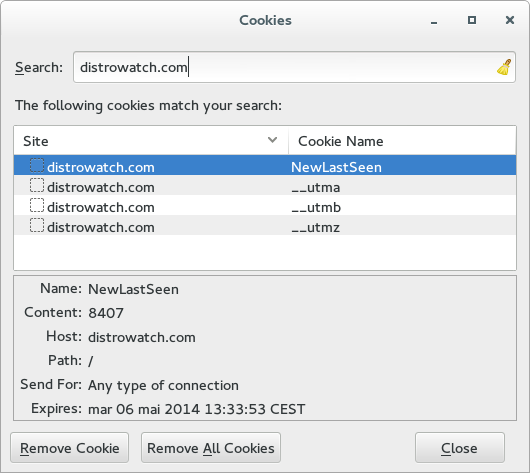
\includegraphics[scale=0.7]{figures/cookies_distrowatch.png}
	\caption{\label{cookies_distrowatch}Les cookies enregistrés pour l'hôte \textit{distrowatch.com} dans Firefox.}
\end{figure}


%%%%%%%%%%%%%%%%%%%%%%%%%%%%%%
\section{Comment le Web est-il censé fonctionner ?}
Lors du chargement d'une page web, le navigateur effectue de multiples connexions afin de récupérer l'ensemble des ressources de la page. Aux débuts du World Wide Web, toutes les ressources d'une page appartenaient généralement à une même personne/groupe. A l'heure actuelle, la situation a fort changé : il est fréquent de voir des ressources chargées depuis des domaines tiers (régies publicitaires, CDN,...). Le navigateur effectue donc des connexions vers des serveurs différents (cela permet notamment de passer outre la limitation du nombre de connexions HTTP vers un même domaine \cite{IETF_RFC2616}) mais en contrepartie, cela permet aux serveurs en question d'enregistrer des données sur le client suite aux requêtes qu'il effectue.


%%%%%%%%%%%%%%%%%%%%%%%%%%%%%%
\section{Principe de même origine}
Le principe de même origine (\textit{same-origin principle}) peut être déclaré comme suit : "seul le site qui enregistre des données dans le navigateur peut lire ou modifier ces données plus tard" \cite{Jackson:2006:PBS:1135777.1135884}.
\newline

Lors du développement de Netscape Navigator 2, une décision importante a été prise concernant le principe de même origine. Celui-ci interdit des sites web de domaines différents d'interagir entre eux au niveau du cache du navigateur, sauf dans des cas précis. Ce principe est implémenté dans les différents navigateurs mais il n'est appliqué de la même manière. En effet, le principe n'a ni été déclaré de manière générale ni appliqué de manière uniforme aux multiples manières dont un site web peut sauvegarder ou récupérer des données de la machine d'un utilisateur.
\newline

L'échec de l'adaptation de ce principe est une source importante de fuites de données.


\chapter{Moyens d'identification}
Dans ce chapitre, nous allons nous intéresser aux techniques qui permettent de tracer les utilisateurs. Plus précisément, nous allons voir comment ces techniques utilisent ou détournent les mécanismes assurant le fonctionnement du Web.

\section{Imperfections du principe de même origine}
L'échec de l'adaptation de ce principe est une source importante de fuites de données et d'attaques. Les violations du principe de même origine peuvent être dues à un filtrage de script insuffisant du côté des applications Web du serveur ou à des défauts dans les mécanismes d'isolation des domaines au sein du navigateur \cite{Chen:2007:ABD:1315245.1315248}.

Les défauts de filtrage des scripts au niveau des serveurs sont communément appelés failles XSS (\textit{cross-site scripting}). En exploitant ces failles, des scripts malveillants peuvent passer à travers le filtrage et être exécutés dans le même contexte de sécurité que les applications Web authentiques.

Au niveau des navigateurs Web, les violations du principe de même origine sont dues à une mauvaise isolation des contenus des différents domaines. Certains domaines peuvent alors accéder aux informations appartenant à d'autres domaines alors qu'ils ne devraient pas y avoir accès.
\newline

L'échec de l'adaptation de ce principe est une source importante de fuites de données. Il faut toutefois noter que s'il était largement appliqué, ce principe changerait énormément de fonctionnalités du Web incluant des choses simples telles que les liens hypertextes entre sites et le contenu intégré.
\newline

Il faut également préciser que même si le principe était correctement implémenté au sein d'un navigateur, il n'empêcherait pas les violations de vie privée face à des sites coopérants. Ceci s'explique par le fait qu'il existe une multitude de techniques simples allant des redirections jusqu'aux liens inter-sites pouvant être utilisées dans le but de transmettre des données entre des sites. Avec de tels échanges, les sites coopérants sont dans la capacité de constituer un profil inter-domaine des activités de leurs visiteurs.
\newline

La possibilité de violer le principe de même origine est la source de nombreuses méthodes qui permettent de tracer les utilisateurs.
En effet, elle permet à un site A de créer et récupérer un cookie sur l'ordinateur de l'utilisateur s'il visite un autre site B qui inclut du contenu du site A (\autoref{cookies}). Cela autorise également des sites à accéder à des éléments d'un autre site enregistrés en cache (\autoref{cache}).

L'absence d'implémentation du principe de même origine dans l'historique de l'utilisateur permet de déterminer si le navigateur a été utilisé pour visiter un site en regardant la couleur des liens hypertextes pointant vers ce site. Dans ce cas, l'utilisation de cookies n'est même plus nécessaire.
\newline

Le traçage des utilisateurs peut être classé en plusieurs catégories \cite{Jackson:2006:PBS:1135777.1135884} :
\begin{itemize}
  \item tracking sur une seule session : inévitable vu comment le Web fonctionne
  \item tracking sur de multiples sessions : permet à un site d'identifier un visiteur s'il revient plus tard sur le site
  \item tracking coopératif : permet à des sites coopérants de créer un historique des visites d'un utilisateur sur tous les sites de la coopération
  \item tracking semi-coopératif sur un seul site : permet à un site de déterminer des informations sur les activités d'un visiteur sur un autre site en y plaçant du contenu (par exemple, en plaçant une image sur un forum)
  \item tracking semi-coopératif sur de multiples sites : identique au tracking semi-coopératif sur un seul site à l'exception qu'il peut y avoir plusieurs sites ciblés
  \item tracking non coopératif : permet à un site de déterminer des informations sur les activités d'un visiteur sur un autre site sans participation du site ciblé
  \newline
\end{itemize}

Certains types de tracking peuvent être évités en améliorant le principe de même origine mais il est malheureusement difficile de contrer les types de tracking dits coopératifs.

%%%%%%%%%%%%%%%%%%%%%%%%%%%%%%
\section{Cookies}
\label{cookies}
En ce qui concerne les cookies, il est assez simple de tracer la navigation d'un utilisateur. En effet, nous avons vu que le navigateur envoie dans chaque requête HTTP un en-tête \textit{Cookie}. Il est donc aisé pour le site web de suivre le parcours du visiteur simplement en analysant cet en-tête. Le fait de passer par un proxy ne change rien car le cookie reste indépendant du moyen d'accès au site web.
\newline

En général, on utilise deux types de classification pour les cookies \cite{Yue:2007:ACU:1251984.1253093}.

Le premier se base sur l'origine et la destination : les cookies sont classifiés en tant que cookies "first-party" ou "third-party". Les cookies "first-party" sont issus du domaine que l'utilisateur est en train de visiter, on les appelle cookies d'origine ou cookies de domaine. Les cookies "third-party" sont créés par un site autre que celui qui est visité par l'utilisateur, on les appelle cookies tiers.

La seconde méthode de classification se base sur la durée de vie du cookie : les cookies sont alors classifiés en cookies de session ou cookies persistants. Les cookies de session sont stockés dans la mémoire vive de l'ordinateur et supprimés à la fermeture du navigateur. A l'opposé, les cookies persistants sont stockés sur le disque dur de l'ordinateur et supprimés soit lors de leur expiration, soit manuellement par l'utilisateur.
\newline

Les cookies tiers, qu'ils soient de session ou persistants, n'apportent quasiment aucun bénéfice à l'utilisateur. Ils sont d'ailleurs reconnus comme une menace pour la vie privée et les navigateurs proposent généralement une option pour les désactiver.

Les cookies d'origine de type session ne posent pas vraiment de problèmes relatifs à la vie privée étant donné leur faible durée de vie.

A l'opposé, les cookies d'origine persistants peuvent poser des problèmes divers. En effet, les cookies persistants sont une arme à double tranchant : ils peuvent jouer un rôle utile en permettant la personnalisation et l'authentification sur les sites mais ils peuvent également jouer un rôle plus dangereux qui amène des risques au niveau de la vie privée et de la sécurité. Ces risques reposent sur deux aspects : le premier, et celui qui nous intéresse principalement ici, est que les cookies persistants permettent de tracer l'activité de l'utilisateur. Le deuxième risque est qu'ils peuvent être volés ou manipulés par des attaques de deux types : les attaques XSS (elles exploitent les vulnérabilités des applications Web) et les attaques qui exploitent les vulnérabilités des navigateurs Web (via notamment le contournement du principe de même origine).
\newline

Une étude menée sur plus de 5000 sites à propos de l'utilisation des cookies \cite{Yue:2007:ACU:1251984.1253093} a montré que les cookies d'origine persistants sont largement utilisés et que plus de 60\% sont réglés pour expirer plus d'un an après leur création.
\newline

Désactiver tous les cookies tiers et garder les cookies d'origine de type session est supporté par la majorité des navigateurs actuels. Le problème se situe au niveau des cookies d'origine persistants car on ne sait pas comment les gérer et déterminer s'ils sont utiles ou néfastes pour l'utilisateur.

%- parler des cookies de cache dans la section cookies ou dans la section cache ?

%%%%%%%%%%%%%%%%%%%%%%%%%%%%%%
\section{Cache}
\label{cache}
Le cache du navigateur permet d'enregistrer localement une copie des fichiers afin de ne pas devoir les recharger lors d'une visite ultérieure. Ce mécanisme est très utile car il permet d'économiser de la bande passante et du temps. Cependant, il donne la possibilité à des sites web de déterminer si leurs visiteurs ont visité un autre site auparavant.

L'exploitation du cache à des fins de surveillance est détaillé par Felten et Schneider \cite{Felten:2000:TAW:352600.352606}.
Le principe est assez simple : il exploite le fait qu'un fichier présent en cache sera chargé beaucoup plus rapidement qu'un fichier qui ne l'est pas. Donc en mesurant le temps d'accès au fichier, il est possible de déterminer si une personne a déjà visité le site web (ou plus précisément, la page) qui utilise ce fichier. En effet, rien n'empêche un site web de charger un fichier hébergé par un autre site.
\newline

Imaginons que l'administrateur d'un site \emph{(alpha.com)} veuille savoir si ses visiteurs se sont également rendus sur un autre site \emph{(beta.com)}. La première chose qu'il doit faire est de se rendre sur le site qu'il veut cibler et choisir un fichier statique pouvant être mis en cache et qui est chargé par tout visiteur (un logo par exemple). Ensuite, le but est de mesurer le temps d'accès du fichier cible.

Le plus fiable et facile est d'utiliser un applet Java ou un JavaScript qui va mesurer le temps de chargement du fichier à partir de son URL. Même si l'utilisateur a désactivé l'exécution de Java et de JavaScript, il est possible d'obtenir une mesure suffisamment précise en chargeant les fichiers suivants dans l'ordre :

\begin{enumerate}
  \item un fichier du site \emph{alpha.com}
  \item le fichier cible du site \emph{beta.com}
  \item un autre fichier du site \emph{alpha.com}
\end{enumerate}

En soustrayant les moments auxquels le serveur reçoit les requêtes des fichiers 1 et 3, l'administrateur du site \emph{alpha.com} est en mesure d'avoir une approximation du temps qu'il a fallu pour charger le fichier 2 (celui de \emph{beta.com}).

Il faut néanmoins respecter certains critères pour que cela fonctionne : forcer le chargement des fichiers de manière séquentielle et de manière invisible en n'altérant pas l'apparence de la page afin que le client ne remarque rien.
\newline

Il est possible d'améliorer la probabilité de distinguer correctement les succès des défauts de cache en effectuant différentes mesures, ce qui permet alors de raffiner les seuils de discrimination : refaire plusieurs fois la mesure d'un même fichier (à partir de la seconde tentative, le fichier sera présent dans le cache) pour les succès de cache et utiliser l'URL de fichiers n'existant pas pour les défauts de cache.

Afin d'améliorer la précision, il est également intéressant de combiner les résultats de plusieurs fichiers mesurés individuellement.
\newline

D'une manière semblable, ce type d'attaque peut également être réalisé sur le cache du DNS. Felten et Schneider ont vérifié la précision des tests avec l'aide de 3 serveurs distincts situés à des distances différentes.

Plus le serveur est situé à une grande distance, plus la requête DNS prend de temps. Les tests ont montré que la précision des résultats pouvait être inférieure car la pénalité suite à des défauts de cache était très petite. Il n'était donc pas possible de discriminer les échecs des succès de cache. Cependant, sur Internet, la pénalité en cas de défaut est suffisamment grande pour assurer une bonne distinction. Dans ce cas-là, les tests montrent une très bonne précision.
\newline

% Attache de cookies de cache

Cette attaque peut être menée dans différentes situations :
\begin{itemize}
  \item Un site web qui veut en savoir davantage sur ses visiteurs.
  \item Une régie publicitaire pourrait inclure le code de mesure dans les bannières qu'elle distribue afin de faire des statistiques sur les sites web consultés par les visiteurs.\\Il est même possible de distribuer un code différent pour les catégoriser.
  \item L'attaquant pourrait créer un site web de telle façon à ce qu'il apparaisse en tête des moteurs de recherche dans le but de faire des statistiques sur les personnes intéressées par un sujet particulier.
  \item L'attaquant pourrait envoyer un mail contenant le code HTML à sa victime.\\En le faisant ressembler à du spam, la victime ne remarquerait rien d'anormal et la mesure serait effectuée.
\end{itemize}

% Timing Attacks on Web Privacy (section 1) : raisons de s'inquiéter
% Timing Attacks on Web Privacy (section 7) : contre-mesures actuelles sont inefficaces
% Timing Attacks on Web Privacy (section 8) : solution possible


%%%%%%%%%%%%%%%%%%%%%%%%%%%%%%
\section{Pixels espions}
Les pixels espions sont des images de taille minime (généralement, de 1 pixel de haut sur 1 pixel de large) et sont destinés à effectuer une requête HTTP vers un serveur sans que le visiteur de la page ne s'en aperçoive. L'administrateur du site hébergeant ce pixel espion peut dès lors analyser les logs de son serveur Web afin d'obtenir des informations sur l'utilisateur. En plaçant un pixel espion spécifique sur chaque site, l'administrateur peut distinguer sans problème les requêtes provenant des différents sites et ainsi déterminer quel site a été visité par chaque utilisateur. De plus, en analysant la requête, il peut connaître l'heure à laquelle le visiteur s'est rendu sur la page mais également d'autres informations telles que le navigateur utilisé, le système d'exploitation, etc.

%%%%%%%%%%%%%%%%%%%%%%%%%%%%%%
\section{JavaScript}
JavaScript permet d'exécuter des scripts du côté client. Il a entraîné le déploiement d'applications riches et accessibles simplement via un navigateur Web. Les possibilités sont multiples : il est ainsi facile de se divertir grâce à un jeu écrit en JavaScript mais il est également aisé d'en savoir plus sur l'utilisateur via le navigateur qui exécute le script. Ceci est possible grâce à l'accès dont dispose JavaScript sur l'ordinateur du client. En effet, différents attaques peuvent être perpétrées avec JavaScript afin d'identifier les utilisateurs \cite{Jang:2010:ESP:1866307.1866339}.
\newline

\begin{itemize}
	\item Le vol de cookies : le script inclus depuis un site tiers a accès à toutes les informations présentes sur la page. Lorsque celle-ci fait appel à un script, elle lui donne accès aux cookies, à la barre d'adresses et à l'ensemble des éléments disponibles sur la page. Le script a donc la capacité de lire le contenu des cookies associés au site et de l'envoyer à un site tiers (une régie publicitaire par exemple).
	\item Le détournement d'adresse : le script, ayant l'accès complet au contenu de la page, peut influencer les valeurs des URL. Le script peut également rediriger le navigateur vers un autre site et le rediriger ensuite vers le site d'origine sans que l'utilisateur ne s'en aperçoive (au chargement de la page par exemple).
	\item L'analyse de l'historique : l'attaque consiste à regarder comment les liens sont affichés par le navigateur. En effet, s'ils ont été visités, les liens s'affichent d'une autre couleur. Il suffit alors de créer un lien vers le site que l'on désire cibler dans une partie invisible de la page et utiliser l'interface DOM du navigateur pour regarder comment celui-ci affiche le lien. Cette attaque est possible car dans la plupart des navigateurs, l'accès à un historique de pages visitées, de fichiers cachés et de cache DNS est partagé entre les domaines.
	\item Le traçage de comportement : il est possible de déterminer avec précision le comportement de l'utilisateur sur la page qu'il visite. L'élaboration d'une ligne du temps avec les interactions de l'utilisateur (clics, mouvements, défilements, parties de texte surlignées,...) est réalisable avec l'aide de gestionnaires d'événements. Cet ensemble d'interactions peut alors être envoyé à un site tiers afin de calculer des statistiques sur la navigation de l'utilisateur.
\end{itemize}

\subsection{Régies publicitaires sur Internet}

\subsection{Modules des réseaux sociaux}
Les réseaux sociaux proposent généralement de placer un plugin social qui permet aux visiteurs d'un site d'interagir et de partager avec leurs amis. Bien sûr, l'intégration d'un tel script permet aux plateformes de réseaux sociaux de suivre la navigation des visiteurs d'un site. Si beaucoup de sites intègrent ces scripts, les réseaux sociaux sont alors en mesure d'obtenir une sorte de carte d'Internet avec les déplacements et actions de chaque utilisateur. De plus, si un visiteur est connecté à son compte sur un réseau social en naviguant sur d'autres sites, la plateforme peut directement faire le lien entre son profil et les sites qu'il visite.

\subsubsection{Facebook}
Le code que les gestionnaires de sites Web doivent intégrer au sein de leur page afin d'accéder aux fonctionnalités offertes par Facebook \cite{javascript_facebook_sdk} est visible à la \autoref{js_facebook_sdk}.

\begin{figure}[h]
	\centering
	\lstinputlisting{examples/js_facebook_sdk}
	\caption{\label{js_facebook_sdk}Le SDK de \textit{Facebook} pour JavaScript}.
\end{figure}

\subsubsection{Google+}
De son côté, Google propose différents scripts à ajouter en fonction des fonctionnalités que le gestionnaire de site Web veut intégrer au sein de sa page (voir \autoref{js_google_plus}). Google propose même de charger de façon asynchrone son script afin d'obtenir des performances optimales (voir \autoref{js_google_plus_async}) \cite{javascript_google_plus}.

\begin{figure}[h]
	\centering
	\lstinputlisting{examples/js_google_plus}
	\caption{\label{js_google_plus}L'API JavaScript de \textit{Google+}}.
\end{figure}

\begin{figure}[h]
	\centering
	\lstinputlisting{examples/js_google_plus_async}
	\caption{\label{js_google_plus_async}L'API JavaScript de \textit{Google+} pour un chargement asynchrone}.
\end{figure}

\subsubsection{LinkedIn}
LinkedIn propose également une API pour connecter les sites avec sa plateforme \cite{javascript_linkedin}. Dans la \autoref{js_linkedin}, on peut même voir que le nom de l'utilisateur (s'il est connecté sur la plateforme) est affiché sur le site. Cet aspect semblera convivial à la majorité des utilisateurs mais cela permet surtout de mieux les suivre lors de leur navigation sur les sites intégrant ce module social.

\begin{figure}[h]
	\centering
	\lstinputlisting{examples/js_linkedin}
	\caption{\label{js_linkedin}L'API JavaScript de \textit{LinkedIn}}.
\end{figure}

\subsection{Outils destinés aux webmasters}
Certaines plateformes proposent aux gestionnaires de sites Web de suivre la navigation des visiteurs sur leur site. Elles regardent d'où viennent les visites (moteur de recherche, accès direct, lien d'un autre site,...), leur navigateur (la version, les plugins installés, la langue,...), sur quels pages les visiteurs se rendent, combien de temps ils restent sur chaque page, etc.

\subsubsection{Google Analytics (Universal Analytics)}
\label{google_analytics}
Une des principales plateformes de suivi des utilisateurs est Google Analytics. Cet outil est utilisé par de nombreux gestionnaires de sites afin de connaître les statistiques de fréquentation de leur site \cite{javascript_google_analytics}.

Comme on peut le voir sur la \autoref{Google_Analytics_1}, les statistiques sont très détaillées. Dans la \autoref{Google_Analytics_2}, la ville des visiteurs était affichée mais il est également possible de voir d'autres données telles que leur FAI ou leur système d'exploitation. Des données spécifiques aux clients mobiles sont également disponibles. Toutes les données sont affichées dans des graphiques clairs et dynamiques et il est même possible d'exporter l'ensemble de ces données dans différents formats (CSV, TSV, Excel, PDF,...) afin de les traiter de manière automatique.
\newline

Google a développé une nouvelle version de son outil d'analyse des visiteurs : Universal Analytics. Ce nouvel outil repose sur le même socle que Google Analytics mais il apporte de nouvelles fonctionnalités.

Pour ce nouvel outil, Google propose 3 types de code de tracking en fonction des plateformes visées : la librairie JavaScript \textit{analytics.js} pour les sites Web, les SDK Google Analytics pour les applications mobiles et le \textit{protocole de mesure ("Measurement Protocol")} pour les autres appareils tels que consoles de jeux et les kiosques d'information.
\newline

Alors que Google Analytics identifiait un utilisateur différent en fonction de chaque appareil connecté, Universal Analytics reconnaît un même utilisateur qui utilise plusieurs moyens de se connecter à Internet. Afin d'y parvenir, ils utilisent un identifiant d'utilisateur unique afin d'associer les données reçues d'appareils et de sessions différentes.

Afin d'utiliser cette fonctionnalité, les gestionnaires de sites Web doivent être en mesure de générer un identifiant unique pour chaque utilisateur et l'associer aux données envoyées à Google. Généralement, cet identifiant unique est généré grâce à l'authentification des visiteurs sur un site. Ainsi, lorsqu'un utilisateur se sert de sa tablette et de son ordinateur pour se rendre sur un site et s'il s'y connecte, Google sera en mesure d'identifier ces visites comme provenant d'un seul et même utilisateur et non plus de deux utilisateurs différents.
\newline

En fonction de la version de Google Analytics utilisée, différents cookies sont créés et utilisés afin de suivre les visites des utilisateurs \cite{Google_Analytics_cookies}.
\newline

La nouvelle librairie JavaScript de Google, \textit{analytics.js} crée un cookie d'origine contenant un identifiant anonyme afin de distinguer les utilisateurs. Par défaut, la librairie crée un cookie sur le domaine de plus haut niveau et règle le chemin du cookie sur le niveau racine.

Le cookie créé est :
\begin{itemize}
  \item[$\bullet$] \textbf{\_ga} : cookie avec une date d'expiration de 2 ans destiné à distinguer les utilisateurs.
  \newline
\end{itemize}

L'ancienne libraire JavaScript de Google, \textit{ga.js}, crée 5 cookies d'origine qui permettent de :
\begin{itemize}
  \item déterminer quel domaine est mesuré
  \item distinguer les utilisateurs uniques
  \item se souvenir du nombre et des heures des visites précédentes
  \item se souvenir de l'information sur la source de trafic
  \item déterminer le début et la fin de session
  \item se souvenir des valeurs des variables personnalisées au niveau de l'utilisateur
\end{itemize}

Par défaut, la librairie crée un cookie sur le domaine spécifié dans la propriété du navigateur \textit{document.host} et règle le chemin du cookie sur le niveau racine.

Les cookies créés sont:
\begin{itemize}
  \item[$\bullet$] \textbf{\_\_utma} : cookie avec une date d'expiration de 2 ans destiné à distinguer les utilisateurs et les sessions.
  \item[$\bullet$] \textbf{\_\_utmb} : cookie avec une date d'expiration de 30 minutes destiné à distinguer les nouvelles sessions et visites.
  \item[$\bullet$] \textbf{\_\_utmc} : cookie avec une date d'expiration de fin de session qui n'est plus utilisé dans \textit{ga.js} mais qui permet l'interopérabilité avec \textit{urchin.js} (une librairie encore plus ancienne de Google Analytics, antérieure à \textit{ga.js}).
  \item[$\bullet$] \textbf{\_\_utmz} : cookie avec une date d'expiration de 6 mois destiné à enregistrer les sources de trafic ou de campagne qui explique comment un utilisateur atteint le site.
  \item[$\bullet$] \textbf{\_\_utmv} : cookie avec une date d'expiration de 2 ans utilisé pour sauvegarder les données des variables personnalisées au niveau de l'utilisateur.
\end{itemize}

\begin{figure}[h]
	\centering
	\lstinputlisting{examples/js_google_analytics}
	\caption{\label{js_google_analytics}L'API JavaScript de \textit{Google Analytics}}.
\end{figure}

\begin{figure}[h]
	\centering
	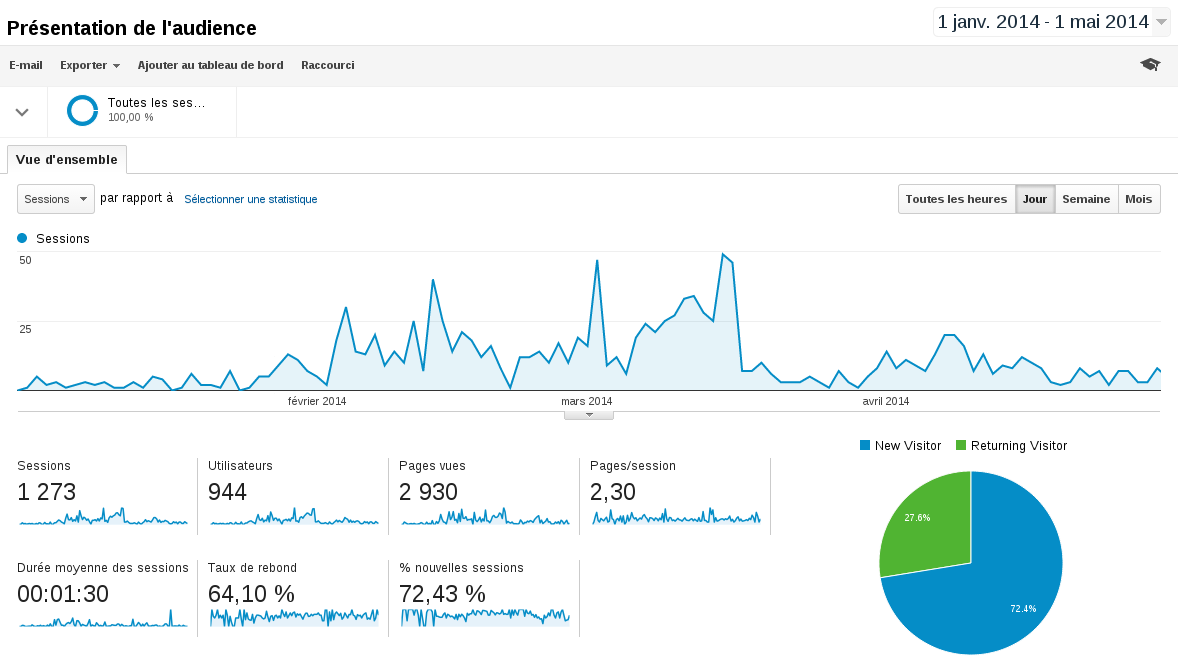
\includegraphics[scale=0.4]{examples/Google_Analytics_1.png}
	\caption{\label{Google_Analytics_1}Copie d'écran de \textit{Google Analytics} qui détaille la navigation sur le site}
\end{figure}

\begin{figure}[h]
	\centering
	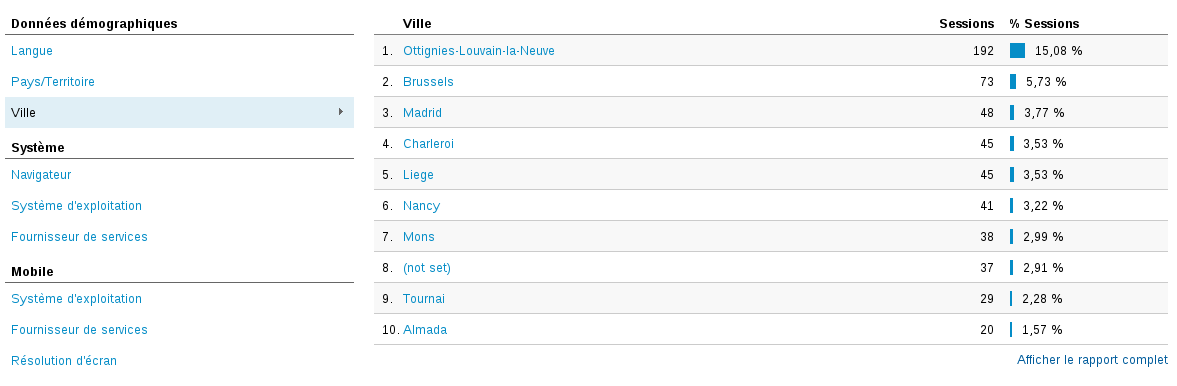
\includegraphics[scale=0.4]{examples/Google_Analytics_2.png}
	\caption{\label{Google_Analytics_2}Copie d'écran de \textit{Google Analytics} qui détaille l'origine des visiteurs}
\end{figure}

%%%%%%%%%%%%%%%%%%%%%%%%%%%%%%
\section{Flash}



%%%%%%%%%%%%%%%%%%%%%%%%%%%%%%
\section{Empreintes des navigateurs}
\label{fingerprinters}



%%%%%%%%%%%%%%%%%%%%%%%%%%%%%%
\section{Conclusion}


\chapter{Analyse des principaux sites web}
\section{Objectif de l'analyse}
Le but de l'analyse est de parcourir les sites les plus visités au monde d'après le classement Alexa \cite{AlexaTop}. Ensuite, déterminer s'ils contiennent des trackers et, le cas échéant, leur nature. Deux types d'expérience peuvent être menés :
\begin{enumerate}
	\item Le premier consiste en une analyse à long terme.
	\item Le second consiste en une analyse ponctuelle.
\end{enumerate}

Le premier type d'expérience a pour but de déterminer si les sites modifient leurs trackers au fil du temps.
Le second type permet d'avoir une image globale du niveau de traçage opéré par les principaux sites à un instant donné. Il donne également la possibilité de tester l'efficacité des extensions de navigateur qui affirment protéger la vie privée (voir \autoref{results_plugins}).

\section{Description de l'outil implémenté}
L'idée initiale était d'utiliser le framework \textit{fpdetective} \cite{Acar:2013:FDW:2508859.2516674}. C'est un framework conçu pour la détection et l'analyse d'outils (\textit{fingerprinters}, voir \autoref{fingerprinters}) qui créent des empreintes de navigateurs. Ce framework semblait prometteur mais son efficacité s'est révélée insuffisante et il ne fonctionnait pas correctement. En effet, aucun \textit{fingerprinter} n'était détecté alors que certains étaient manifestement présents sur plusieurs sites web visités.

Etant donné que \textit{fpdetective} ne pouvait fournir les résultats demandés, la création d'un outil dédié à cette tâche était nécessaire. De plus, cela permettait davantage de souplesse au niveau des décisions d'implémentation et du paramétrage de la recherche de trackers.
\newline

L'outil a été implémenté en Java. Il se compose de deux éléments : le \textit{crawler} qui visite les sites web et exporte leur contenu au format HTTP Archive (HAR) et le \textit{parser} qui traite les fichiers HAR en déterminant si les sites correspondants renferment des trackers.
L'outil a été développé sous Eclipse et est destiné à être utilisé sur Linux. Un exécutable Jar est également disponible.
\newline

Lors du lancement du \textit{crawler}, l'utilisateur peut spécifier plusieurs arguments :
\begin{itemize}
	\item Requis : le mode (\textit{crawler} ou \textit{parser}).
	\item Requis : le répertoire des fichiers.\\
		Pour le \textit{crawler}, il s'agit du répertoire où les fichiers seront enregistrés.\\
		Pour le \textit{parser}, il s'agit du répertoire contenant les fichiers à analyser.
	\item Optionnel : l'activation du mode \textit{debug} qui va donner davantage de détails en cas de problème.
	\item Optionnel : l'affichage de l'aide.
	\newline
	\item Requis pour le \textit{crawler} : le profil de Firefox à utiliser.
	\item Requis pour le \textit{crawler} : le fichier contenant la liste des sites web à visiter.
	\item Requis pour le \textit{crawler} : le début de l'intervalle des sites à visiter.
	\item Requis pour le \textit{crawler} : la fin de l'intervalle des sites à visiter.
	\item Requis pour le \textit{crawler} : le nombre maximal de tentatives par site web (\textit{timeout}).
	\item Requis pour le \textit{crawler} : le nombre de sites à visiter avant le redémarrage de Firefox.
	\newline
	\item Requis pour le \textit{parser} : le fichier contenant la liste des trackers de Ghostery.
	\item Optionnel pour le \textit{parser} : l'activation de l'impression de tous les trackers identifiés.
\end{itemize}

\subsection{Crawler}
\label{crawler}
\subsubsection{Choix d'implémentation}
Afin d'automatiser le navigateur et de parcourir les sites sans intervention humaine, \textit{Selenium} \cite{selenium_homepage} est utilisé. Plus précisément, c'est le pilote \textit{FirefoxDriver} de \textit{Selenium} qui est utilisé au sein de l'outil.

La première implémentation traitait directement le code source de la page. Il était possible d'aller sur le moteur de recherche Google, de sélectionner le champ de recherche, de taper une requête et de récupérer le résultat. Cependant, le processus était assez lent et incomplet car on ne pouvait pas récupérer les requêtes et les réponses HTTP. On pouvait juste récupérer les éléments associés à des balises (par exemple, récupérer toutes les images via les balises de type \textit{<img>}, les scripts avec les balises \textit{<script>},...) mais tout n'était pas récupérable car certains éléments étaient chargés sans être identifiés.

Afin de pallier ce problème, la deuxième implémentation utilisait un proxy qui exportait le contenu du site au format HTTP Archive. L'ensemble des requêtes et réponses HTTP était récupéré et enregistré dans un fichier. Le parcours du code source (qui donnait des résultats finalement incomplets) a été supprimé afin de rendre le programme plus rapide. Cette fois, le problème était que le proxy n'exécutait pas le JavaScript. Il en résultait que de nombreux sites ne pouvaient être chargés correctement (cela pouvait varier de 15 à 30\% d'échecs) et il était alors impossible de les traiter.

La troisième solution, qui est la dernière implémentée, consiste à utiliser le pilote pour charger les sites automatiquement, sans parcours du code source ni utilisation de proxy. Le contenu des sites est exporté au format HTTP Archive à l'aide de deux extensions qui ont été installées dans Firefox.
\begin{itemize}
	\item La première, Firebug \cite{firebug_homepage}, est une extension utilisée principalement par les développeurs de sites web afin de les débugger. Elle permet de monitorer les éléments d'une page (CSS, HTML, JavaScript) en direct.
	\item La seconde, NetExport \cite{netexport_homepage}, est une extension de Firebug qui permet d'exporter toutes les données d'une page au format HTTP Archive de façon automatique (il est possible de paramétrer cette extension pour le faire).
\end{itemize}

Le taux de réussite de l'export des données des sites s'est grandement amélioré. Néanmoins, certains sites ne sont toujours pas chargés correctement.
Une hypothèse est que certains sites sont hébergés sur des serveurs lointains et leurs éléments prennent alors plus de temps à charger. Ainsi, lorsque ces sites contiennent une grande quantité d'éléments, le pilote renvoie une exception de type \textit{timeout} et le chargement du site est finalement en échec. On remarque généralement ceci sur les sites asiatiques : certains portails regorgent de contenus qui prennent du temps à charger.
Une hypothèse supplémentaire est que certains sites demandent une action de l'utilisateur (faire défiler la page par exemple) afin de charger les éléments du site (typiquement, les images).
\newline

Une amélioration a été apportée à l'outil afin de compter le nombre de cookies Flash et de cookies classiques (qu'ils soient enregistrés via les réponses HTTP ou des scripts JavaScript) lors de chaque visite de site. Cette fonctionnalité a été implémentée au sein du \textit{crawler} étant donné que ce n'est pas possible d'accéder à cette information avec l'aide des fichiers HTTP Archive analysés par le \textit{parser}. Cela signifie qu'une partie des résultats est déjà disponible lorsque le \textit{crawler} a fini de visiter les sites.

A son lancement, il supprime l'ensemble des cookies Flash (les fichiers .sol) dans le dossier \textit{.macromedia/Flash\_Player/\#SharedObjects/XXXXXXXX/}. Il supprime également les cookies Firefox en se connectant à la base de données SQLite dans \textit{.mozilla/firefox/<profil>/cookies.sqlite} et en vidant la table \textit{moz\_cookies}. Cela permet de s'assurer que la visite des sites ne sera pas influencée par la présence de cookies antérieurs.

\subsubsection{Changements opérés sur les extensions}
\label{changements_extensions}
Deux modifications ont été nécessaires sur l'extension \textit{NetExport} de \textit{Firebug}.

La première concerne la génération des fichiers HTTP Archive. Par défaut, l'extension ajoute un champ qui n'est pas standard par rapport à la spécification du format HAR. Il en résulte que les fichiers peuvent alors être considérés comme corrompus alors que la présence ou non de ce champ n'influence en rien les résultats qui nous concernent. La génération de ce champ a donc été supprimée dans le fichier \textit{/chrome/content/netexport/harBuilder.js} de \textit{NetExport}.

La seconde modification concerne le nom des fichiers générés. Par défaut, l'extension ajoute la date à l'URL du site dans les noms de fichier. Cela pose des difficultés supplémentaires au \textit{parser} lors de la récupération et du traitement de ces fichiers (voir \autoref{parser}). L'extension a donc été modifiée afin de n'utiliser que l'URL du site dans les noms du fichier. Cette modification a été effectuée dans le fichier \textit{/chrome/content/netexport/automation.js}. Sur Linux, lorsqu'un fichier de même nom existe déjà, un tiret suivi du numéro de copie est ajouté au nom de fichier avant son extension.

\subsubsection{Fonctionnement}
Le \textit{crawler} fonctionne de la manière suivante. D'abord, il vérifie que le répertoire donné en argument est accessible en écriture et il crée deux dossiers nommés "logs" et "results" qui sont destinés à contenir respectivement les logs et les résultats du \textit{crawler}. Ensuite, le fichier de log (log\_crawler.txt) est créé, le dossier des cookies Flash est détecté (s'il y en a plusieurs, l'utilisateur est invité à indiquer le bon dossier) et la base de données SQLite des cookies Firefox est vidée (le dossier des paramètres de l'utilisateur est automatiquement trouvé grâce au profil Firefox spécifié en argument au lancement du programme). La liste des sites à visiter est ainsi chargée depuis le fichier spécifié et en fonction de l'intervalle donné par l'utilisateur. Puis, le profil Firefox choisi est chargé et différents paramètres de configuration des extensions sont également réglés avant que le pilote ne soit initialisé et qu'il lance Firefox. Après le lancement du pilote, un délai de 5 secondes laisse le temps à Firefox de se lancer et de charger ses extensions.
\newline

Après cette phase de préparation, le parcours des sites commence. Le pilote dirige Firefox sur l'URL du premier site de la liste. Lorsque le chargement de la page est terminé, un délai de 8 secondes permet aux extensions d'enregistrer le fichier HTTP Archive. Le nombre de cookies Flash est enregistré pour chaque site.

Si la page s'est chargée avant la limite de 30 secondes, l'enregistrement est considéré comme valide et le pilote charge le site suivant dans la liste.

Si un site fait un timeout et que l'utilisateur a précisé un nombre de tentatives supérieur à 1, le pilote dirige Firefox sur la page "about:blank" (cela permet d'éviter des problèmes d'écriture de fichiers avec les extensions) puis le redirige sur le site pour un nouvel essai. Ce processus est répété à chaque timeout jusqu'à atteindre le nombre maximal de tentatives. Si le site fait encore un timeout lors de la dernière tentative, il est alors considéré en échec et son URL est inscrite dans une liste reprenant tous les sites en échec. A la deuxième tentative, l'URL du site a déjà été enregistrée dans une autre liste reprenant tous les sites ayant fait un timeout, cela permet de garder une trace des sites dont la visite a rencontré un problème mais qui ont finalement pu être chargés. 

Il arrive également qu'un site ne puisse tout simplement pas être chargé (à cause d'une erreur dans son code source par exemple). Son URL est alors directement enregistrée dans la liste reprenant les sites en échec.
\newline

Lorsque le parcours de l'ensemble des sites est terminé, le programme efface les fichiers inutiles générés lors de la visite des pages "about:blank" et détaille l'ensemble des sites ayant subi au moins un timeout et les sites en échec. La liste des sites avec leur nombre de cookies Flash est enregistrée en ordre décroissant dans le fichier "stats\_flash-cookies.csv" du dossier "results". Pour terminer, le pilote est arrêté (ce qui entraîne la fermeture de Firefox) et le fichier de log est fermé.
\newline

Il a été nécessaire d'implémenter une fonctionnalité qui redémarre Firefox à intervalles réguliers. En effet, certains sites ouvrent des pop-ups et si le navigateur n'est pas fermé, ces derniers s'accumulent et occupent une part plus importante de ressources. Le redémarrage du navigateur permet de fermer toutes ces fenêtres ouvertes de façon intempestive afin de garantir une meilleure stabilité du \textit{crawler}.

\subsection{Parser}
\label{parser}
\subsubsection{Choix d'implémentation}
Lors de la visite des sites par le \textit{crawler}, il arrive que celui-ci doive refaire de nouvelles visites afin d'exporter correctement le fichier HTTP Archive d'un site. Il en résulte que plusieurs fichiers pour le même site soient disponibles. Par exemple, on peut très bien voir des fichiers tels que \textit{monsite.com.har}, \textit{monsite.com-1.har}, etc. Lors de l'analyse de ces fichiers par le \textit{parser}, celui-ci considère seulement la dernière version du fichier comme étant valide. Il ignore donc les autres fichiers concernant le même site (si jamais il y en a plusieurs) car ils sont généralement corrompus ou incomplets.
\newline

Lors de l'analyse d'un site, l'autorité en charge pour son domaine est automatiquement récupérée via une requête DNS de type SOA. Cela permet de déterminer si une URL présente dans le site appartient au même domaine ou si elle provient d'un domaine différent.

Si l'autorité du site analysé ne peut être récupérée, l'analyse du site est considérée comme étant en échec et le nom du fichier contenant les informations de ce site est ajouté dans une liste reprenant tous les fichiers en échec.

Si l'autorité du domaine d'une URL ne peut être récupérée, l'analyse de cette URL est passée mais l'analyse des URL suivantes du fichier continue. Un message est imprimé dans le log pour préciser que la récupération de l'autorité du domaine d'une URL a subi un problème.

Lorsqu'une URL est constituée d'une adresse IP, l'outil fait une requête DNS afin de connaître le nom associé à cette IP. S'il n'y parvient pas, l'analyse de l'URL est passée mais le processus d'analyse continue comme c'est le cas lorsqu'une autorité ne peut être récupérée pour une URL. Ceci est dû au fait que la libraire utilisée (\textit{dnsjava}) n'est pas en mesure d'effectuer des requêtes SOA pour des adresses IP.

Le fonctionnement de la récupération de l'autorité d'une URL est le suivant : tout d'abord, la requête est effectuée sur l'hôte de l'URL. Si aucune réponse n'est retournée, la requête est effectuée sur le domaine parent et ainsi de suite, jusqu'à trouver une réponse ou arriver au domaine le plus haut.

Un système de mise en cache a été mis en place afin de limiter le nombre de requêtes effectuées et d'améliorer la rapidité d'accès à l'information.

\subsubsection{Limitation des requêtes DNS de type SOA}
Le recours aux informations SOA permet généralement de déterminer si deux sites appartiennent au même domaine. C'est ainsi que lors de la visite de \textit{youtube.com}, les images provenant de \textit{ytimg.com} ne sont pas détectés comme provenant d'un site externe (voir \autoref{dig_youtube} et \autoref{dig_ytimg}).

\begin{figure}[h]
	\centering
	\lstinputlisting[style=dig]{examples/dig_youtube.com}
	\caption{\label{dig_youtube}Informations SOA pour \textit{youtube.com}}.
\end{figure}

\begin{figure}[h]
	\centering
	\lstinputlisting[style=dig]{examples/dig_ytimg.com}
	\caption{\label{dig_ytimg}Informations SOA pour \textit{ytimg.com}}.
\end{figure}
Comme vous pouvez le voir, les sites \textit{youtube.com} et \textit{ytimg.com} sont sous la même autorité qui est \textit{dns-admin@google.com}. Dans ce cas, toute URL présente dans le site \textit{youtube.com} provenant de \textit{ytimg.com} ne sera pas considérée comme extérieure au site.
\newline

Cependant, il peut y avoir des faux positifs résultant des réponses reçues. C'est ainsi que lors des analyses, un phénomène a été remarqué: à certains moments, la requête DNS peut renvoyer une réponse différente. Ceci a été remarqué pour le site \textit{p8.qhimg.com} (voir \autoref{dig_p8.qhimg.com_1} et \autoref{dig_p8.qhimg.com_2}). Dans ce précis, la requête DNS précise que l'autorité du site est en fait celle de l'hébergeur de contenu \textit{cloudfront.net} (qui est lui-même hébergé sur les serveurs d'\textit{Amazon}) et non plus celle du site visité. Cela dépend en fait de l'infrastructure de leur hébergement et ceci ne pourrait être pris en compte au sein de l'outil sans ralentir de façon conséquente ses performances.

\begin{figure}[h]
	\centering
	\lstinputlisting[style=dig]{examples/dig_p8.qhimg.com_1}
	\caption{\label{dig_p8.qhimg.com_1}Informations SOA pour \textit{p8.qhimg.com}}.
\end{figure}

\begin{figure}[h]
	\centering
	\lstinputlisting[style=dig]{examples/dig_p8.qhimg.com_2}
	\caption{\label{dig_p8.qhimg.com_2}Informations SOA pour \textit{p8.qhimg.com}, 10 secondes plus tard}.
\end{figure}

\subsubsection{Critères qualifiant un tracker}
Le \textit{parser} parcourt l'ensemble des requêtes et réponses HTTP effectuées lors du chargement du site. Afin de déterminer si une ressource chargée est un tracker, l'outil se base sur plusieurs critères.
\begin{itemize}
  \renewcommand{\labelitemi}{$\Rightarrow$}
 \item Présence de l'URL dans la base de données de trackers Ghostery
 \item Si l'URL n'est pas présente dans la base de données Ghostery, l'autorité du domaine de l'URL est récupérée et comparée à celle du site visité.\\
		Si les autorités sont différentes, les critères suivants permettent de déterminer si l'URL est un tracker:
		\begin{itemize}
			\item Un cookie est créé via la réponse HTTP
			\item La ressource chargée est du JavaScript
			\item La ressource chargée est du Flash
			\item Les images chargées ont une largeur et hauteur de 1 pixel (pixels espions)
			\item L'URL des ressources chargées contient des paramètres
			\newline
		\end{itemize}
\end{itemize}

Afin de pouvoir utiliser la base de données Ghostery \cite{ghostery_homepage}, un contact a été pris avec Evidon (les développeurs de l'extension) qui a donné son autorisation d'utiliser la base de données au sein de cet outil.
\newline

Il est évident que certains de ces critères peuvent mener à des faux positifs mais potentiellement chaque ressource chargée d'un site externe permet de tracer l'utilisateur. Dans ses logs, l'administrateur d'un site peut déterminer à quelle heure et quelle ressource un utilisateur a demandé (cela est particulièrement utilisé par les pixels espions).

Au-delà de cette première donnée, l'administrateur du site peut également enregistrer un cookie sur l'ordinateur de l'utilisateur afin de l'identifier s'il recharge une ressource du serveur ultérieurement.

Le fichier JavaScript provenant d'un site externe peut également créer des cookies sans l'autorisation du site qui fait appel à ce script.

Le chargement de ressources contenant des paramètres repose sur le même principe que l'analyse des logs sauf qu'il permet d'aller plus loin en précisant un identifiant pour chaque site qui souhaite charger des ressources d'un autre site.

\subsubsection{Fonctionnement}
Le but du \textit{parser} est de traiter les fichiers HTTP Archive générés par le \textit{crawler} et de déterminer le nombre de trackers pour chaque site. La première chose qu'il fait à son lancement est de vérifier que le dossier donné en argument est accessible en écriture. Il regarde ensuite si des dossiers "logs" ou "results" sont déjà présents et si ce n'est pas le cas, il les crée. S'ils sont déjà présents, le \textit{parser} avertit l'utilisateur qu'il va les utiliser afin d'y écrire des données. Concernant le dossier "results", il demande à l'utilisateur s'il souhaite continuer car des fichiers provenant de résultats calculés antérieurement pourraient être écrasés. Puis, le \textit{parser} ouvre un fichier de log ("log\_parser.txt" dans le sous-dossier "logs"). Ensuite, il charge l'ensemble des sites comme expliqué ci-dessus, il ouvre le fichier contenant la base de données de trackers Ghostery et charge l'ensemble des expressions régulières utilisées afin de détecter les trackers. L'analyse des fichiers HTTP Archive commence et exporte pour chaque site analysé de multiples informations telles qu'expliqué dans la sous-section précédente. Lorsque tous les fichiers ont été analysés, le \textit{parser} calcule les statistiques pour l'ensemble de l'analyse. Ensuite, il indique le nombre de fichiers ayant été correctement analysés et détaille les fichiers n'ayant pu être traités. Pour terminer, il ferme le fichier de log.

\subsection{Format des résultats}
Il existe deux types de résultats : les résultats détaillés pour chaque fichier HTTP Archive analysé et les résultats globaux de l'analyse.

Les résultats globaux sont enregistrés dans le dossier "logs" alors que les résultats détaillés sont enregistrés dans le dossier "results".
Ceci a été décidé par souci de simplicité car les résultats globaux sont ainsi directement accessibles et ne sont pas noyés dans le dossier contenant les résultats détaillés.

\subsubsection{Crawler}
Les résultats globaux dans le dossier "logs" :
\begin{itemize}
	\item \textbf{stats\_flash-cookies.csv} contient la liste des sites utilisant des cookies Flash, triés par ordre décroissant.
	%\newline
\end{itemize}

\subsubsection{Parser}
Les résultats globaux dans le dossier "logs" :
\begin{itemize}
	\item \textbf{stats\_detailed.csv} contient la liste des sites avec le nombre détaillé de trackers (trackers connus identifiés avec l'aide de Ghostery, réponses HTTP créant un cookie, fichiers JavaScript avec ou sans paramètres chargés depuis un autre domaine, Flash chargés depuis un autre domaine, pixels espions et requêtes d'URL avec des paramètres).
	\item \textbf{stats\_mimetypes.csv} contient la liste des types d'éléments (\textit{mimetype}) chargés d'un domaine différent, triés par ordre décroissant.
	\item \textbf{stats\_trackers.csv} contient la liste des trackers identifiés grâce à Ghostery, triés par ordre décroissant.
	\newline
\end{itemize}

Les résultats détaillés pour chaque site dans le dossier "results" :
\begin{itemize}
	\item \textbf{<URL du site>\_cookies.csv} contient la liste des cookies créés par des réponses HTTP d'un domaine différent.
	\item \textbf{<URL du site>\_flash.csv} contient la liste des fichiers Flash provenant d'un autre domaine.
	\item \textbf{<URL du site>\_ghostery.csv} contient la liste des trackers détectés grâce à la base de données Ghostery.
	\item \textbf{<URL du site>\_js.csv} contient la liste des fichiers JavaScript provenant d'un domaine tiers.
	\item \textbf{<URL du site>\_js-query.csv} contient la liste des fichiers JavaScript provenant d'un domaine tiers et appelés avec des paramètres.
	\item \textbf{<URL du site>\_mimetypes.csv} contient la liste des types d'éléments (\textit{mimetype}) chargés d'un domaine différent, triés par ordre décroissant.
	\item \textbf{<URL du site>\_parameters.csv} contient la liste des requêtes vers un domaine différent dont l'URL contient des paramètres.
	\item \textbf{<URL du site>\_pixels.csv} contient la liste des pixels espions détectés depuis un autre domaine.
	\item \textbf{<URL du site>\_urls.csv} contient la liste de l'URL de toutes les ressources chargées d'un domaine différent.
	\newline
\end{itemize}

\section{Résultats}

\subsection{Expérience 1 : étude à long terme}
\subsubsection{Détails de l'expérience}
Le but de cette expérience est de déterminer l'évolution des trackers sur une certaine période en effectuant des mesures de façon régulière.

Afin de réaliser cette étude, le \textit{crawler} a été lancé chaque jour du 28 mars au 7 mai 2014 (à l'exception du 8 avril) sur le TOP 1000 du classement Alexa \cite{AlexaTop}, ce qui représente 40 jours de mesures. Notez cependant que l'implémentation du compteur de cookies Flash a été réalisée ultérieurement à cette expérience et ces données ne sont donc pas disponibles au sein de l'expérience.
\newline

Le \textit{crawler} a été lancé avec les paramètres suivants :
\begin{itemize}
	\item les sites visités sont issus du TOP Alexa du 26 mars 2014
	\item l'intervalle sélectionné concerne les 1000 premiers sites
	\item 3 tentatives maximum ont été autorisées par site
	\item Firefox était redémarré tous les 50 sites
	\item Firefox était dépourvu de toute extension (autre que Firebug et NetExport)
	\newline
\end{itemize}

\subsubsection{Premières constatations}
Lors de cette expérience, on peut voir que le taux d'échec avec le \textit{crawler} est toujours inférieur à 9\%.
Notez que l'implémentation a un peu changé depuis cette expérience. Lors de cette dernière, quand un site atteignait le nombre maximum de tentatives et qu'il était placé dans la liste des sites en échec, il était également retiré de la liste des sites ayant eu besoin d'au moins un nouvel essai suite à un timeout.
Ceci explique des situations telles que sur la \autoref{Exp1_crawler_fails} au début du mois de mai.

\begin{figure}[h]
	\centering
	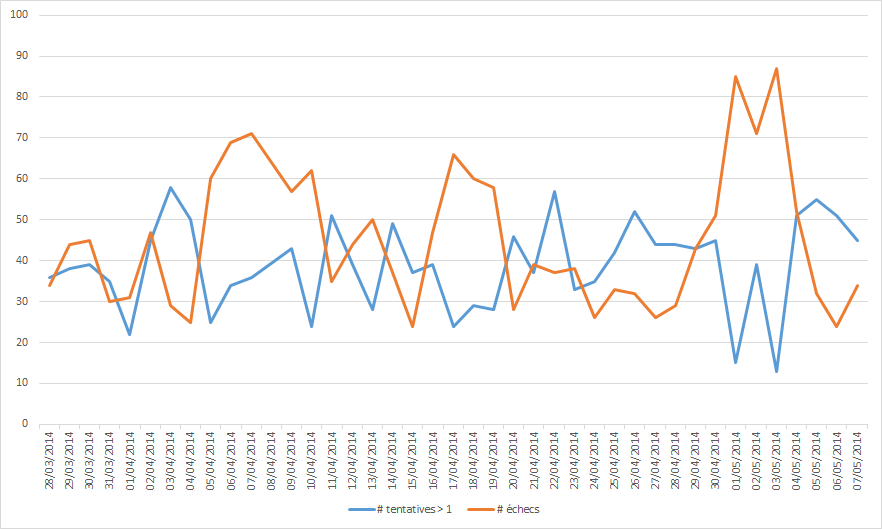
\includegraphics[scale=.7]{graphiques/Exp1_crawler_fails.png}
	\caption{\label{Exp1_crawler_fails}Le nombre d'échecs du \textit{crawler}}.
\end{figure}

\begin{figure}[h]
	\centering
	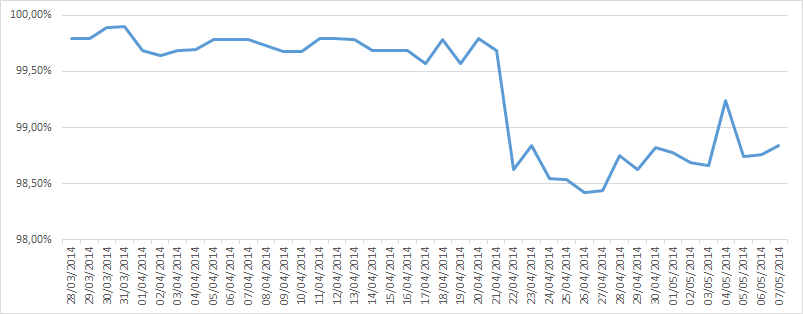
\includegraphics[scale=.8]{graphiques/Exp1_parser_success_rate.png}
	\caption{\label{Exp1_parser_success_rate}Le pourcentage de réussite du \textit{parser}}.
\end{figure}

Le pourcentage de fichiers correctement analysés est représenté à la \autoref{Exp1_parser_success_rate}. On peut voir que du début de l'expérience jusqu'au 21 avril, le pourcentage de réussite est en moyenne de 99,73\%. A partir du 22 avril et jusqu'à la fin de l'expérience, il passe à 98,71\%. Cela représente une dizaine de fichiers.
Croyant d'abord à une erreur lors de l'exécution du \textit{parser}, les analyses ont été reconduites une seconde fois mais n'ont pas montré de résultat différent.
Après analyse des fichiers de log du \textit{parser}, on remarque que ce sont généralement les mêmes sites qui sont en échec.
Ainsi, sur les 16 jours (du 22 avril jusqu'au 7 mai), on peut remarquer certains faits.
\newline
Les sites suivants étaient chaque jour en échec:
\begin{itemize}
  \item 9gag.com
  \item mashable.com
  \item www.pixiv.net
  \item www.wikihow.com
  \newline
\end{itemize}
Les sites suivants n'ont pas été en échec 1 jour :
\begin{itemize}
  \item www.gamespot.com : le 4 mai
  \item www.theverge.com : le 4 mai
  \newline
\end{itemize}
Les sites suivants n'ont pas été en échec 2 jours :
\begin{itemize}
  \item www.thefreedictionary.com : le 25 avril et le 4 mai
  \item www.wix.com : le 28 avril et le 4 mai
  \newline
\end{itemize}
Les sites suivants ont été en échec sur une période de plusieurs jours :
\begin{itemize}
  \item www.rednet.cn : 3 jours (du 25 au 27 avril)
  \item chinaz.com : 2 jours (les 27 et 28 avril)
  \item www.groupon.com : 2 jours (les 5 et 6 mai)
  \newline
\end{itemize}
Les sites suivants n'ont été en échec qu'un seul jour :
\begin{itemize}
  \item www.suning.com : le 22 avril
  \item baomihua.com : le 24 avril
  \item bleacherreport.com : le 26 avril
  \item www.aili.com : le 27 avril
  \item www.hm.com : le 30 avril
  \item www.businessinsider.com : le 3 mai
  \newline
\end{itemize}
Les autres sites en échec ne peuvent pas être classés de manière identique.\\

La constatation que certains sites sont en échec pendant la période complète des 16 jours (alors qu'ils ne l'étaient pas avant le 22 avril) et que certains sites sont en échec sur une courte période (2-3 jours) fait penser que ces échecs résultent d'une erreur située sur les sites eux-mêmes.
\newline

Une recherche approfondie a été effectuée et celle-ci a confirmé l'hypothèse selon laquelle l'erreur provient des données reçues des serveurs. Plus précisément, les erreurs proviennent de champs non reconnus dans les réponses HTTP ou de valeurs erronées. Quelques exemples illustrant les erreurs rencontrées ont été ajoutés.
\newline

\begin{figure}[h]
	\centering
	\lstinputlisting[style=dig]{examples/bad_field_google}
	\caption{\label{bad_field_google}Réponse HTTP de \textit{Google} qui veut créer un cookie avec un champ "priority"}.
\end{figure}

\begin{figure}[h]
	\centering
	\lstinputlisting[style=dig]{examples/bad_field_baidu}
	\caption{\label{bad_field_baidu}Réponse HTTP de \textit{Baidu} avec un champ "domian" au lieu de "domain"}.
\end{figure}

\begin{figure}[h]
	\centering
	\lstinputlisting[style=dig]{examples/bad_field_gamespot}
	\caption{\label{bad_field_gamespot}Réponse HTTP de \textit{GameSpot} avec la valeur "0" pour le champ "expire"}.
\end{figure}

\subsubsection{Nombre de trackers}
Le nombre total de trackers semble rester stable, il est en moyenne de 30080. Ce nombre chute le 2 avril où il est de 25770 trackers. Ceci s'explique par le fait que le nombre de fichiers HTTP Archive pour ce jour (845 fichiers) est inférieur comparé aux autres jours, ce qui fait que moins de sites ont pu être analysés. Le nombre inférieur de fichiers provient probablement d'une perte de données suite à une suppression accidentelle ou à un manque d'espace disque qui a empêché l'enregistrement des fichiers HTTP Archive.

\begin{figure}[h]
	\centering
	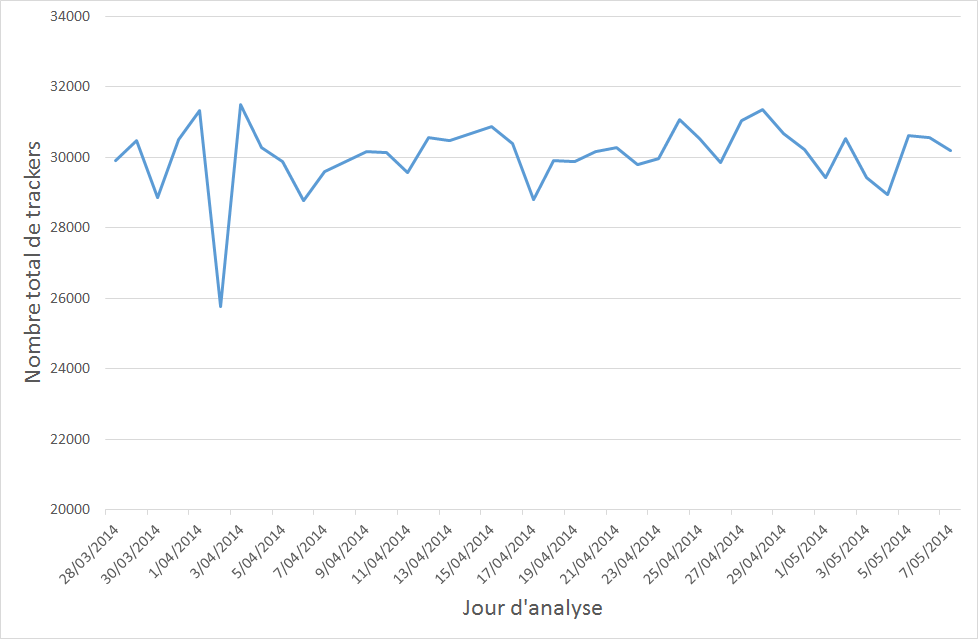
\includegraphics[scale=.8]{graphiques/Exp1_parser_total_trackers.png}
	\caption{\label{Exp1_parser_total_trackers}Nombre total de trackers sur l'ensemble de l'analyse}.
\end{figure}
\subsection{Expérience 2 : étude ponctuelle}
Cette expérience a été lancée de manière ponctuelle afin d'établir une image des sites à un instant donnée. Elle permet aussi de constituer la base de référence pour la comparaison des extensions.
\newline

Le \textit{crawler} a été lancé avec les paramètres suivants :
\begin{itemize}
	\item les sites visités sont issus du TOP Alexa du 16 mai 2014
	\item l'intervalle sélectionné concerne les 1000 premiers sites
	\item 3 tentatives maximum ont été autorisées par site
	\item Firefox était redémarré tous les 50 sites
	\item Firefox était dépourvu de toute extension (autre que Firebug et NetExport)
	\newline
\end{itemize}
Les 36 sites suivants ont été en échec, ce qui signifie qu'aucun fichier HTTP Archive n'a été généré pour eux :
\begin{multicols}{3}
\begin{itemize}
  \item 39.net
  \item aili.com
  \item baomihua.com
  \item bitauto.com
  \item caijing.com.cn
  \item china.com
  \item csdn.net
  \item enet.com.cn
  \item gazeta.ru
  \item gmw.cn
  \item hao123.com
  \item heise.de
  \item howstuffworks.com
  \item ifeng.com
  \item ileehoo.com
  \item justdial.com
  \item kdnet.net
  \item lady8844.com
  \item microsoftonline.com
  \item moz.com
  \item online.sh.cn
  \item onlinesbi.com
  \item opensiteexplorer.org
  \item pchome.net
  \item people.com.cn
  \item pinimg.com
  \item qq.com
  \item secureserver.net
  \item sina.com.cn
  \item sohu.com
  \item tudou.com
  \item twimg.com
  \item yesky.com
  \item yoka.com
  \item youku.com
  \item zing.vn
\end{itemize}
\end{multicols}

Ces sites ne seront par conséquent pas analysés dans cette expérience.
\newline

Par ailleurs, 78 sites ont subi au moins un timeout mais ils ne seront pas listés ici. Notez que si ces sites ont rencontré 3 timeouts consécutifs, ils sont présents dans la liste des sites en échec (ci-dessus).
\newline

Le \textit{parser} a été lancé avec le paramètre suivant :
\begin{itemize}
	\item la base de données Ghostery est la version 300
	\newline
\end{itemize}

Le \textit{parser} n'a pas été en mesure d'ouvrir les fichiers suivants :
\begin{multicols}{2}
\begin{itemize}
  \item 9gag.com.har
  \item accounts.google.com-2.har
  \item mashable.com.har
  \item website-unavailable.com-1.har
  \item www.babytree.com.har
  \item www.deezer.com.har
  \item www.gamespot.com.har
  \item www.gmail.com.har
  \item www.pixiv.net.har
  \item www.thefreedictionary.com.har
  \item www.theverge.com-1.har
  \item www.wikihow.com.har
  \item www.wix.com.har
\end{itemize}
\end{multicols}

Ces sites ne seront par conséquent pas analysés dans cette expérience.
\newline

Les critères retenus pour la classification des trackers sont les suivants :
\begin{itemize}
	\item les URL détectées comme trackers par la base de données Ghostery
	\item les réponses HTTP d'un domaine tiers qui créent un cookie
	\item les requêtes vers un domaine tiers de fichiers JavaScript avec des paramètres
	\item les requêtes de fichiers Flash
	\item les pixels de traçage
	\item les requêtes vers un domaine tiers dont l'URL contient des paramètres
	\newline
\end{itemize}

\subsubsection{Carte des trackers détectés}


\subsubsection{Sites renfermant le plus de trackers détectés}

\subsubsection{Organisations déployant le plus de trackers}
En ne considérant que les trackers détectés par Ghostery, voici la liste des organisations dont le plus de trackers ont été détectés dans cette analyse.
\newline

Sur un total de 24626 trackers :
\begin{itemize}
  \item 2562 sont de DoubleClick
  \item 1379 sont de AppNexus
  \item 949 sont de Google Analytics
  \item 675 sont de Google Adsense
  \item 574 sont de Rubicon
  \item 534 sont de Turn
  \item 441 sont de ScoreCard Research Beacon
  \item 347 sont de MediaMath
  \item 332 sont de Lotame
  \item 326 sont de OpenX
  \newline
\end{itemize}

Quand on sait que DoubleClick appartient à Google, cela fait 4186 cookies provenant de Google qui ont été détectés. Cela représente 17\% des trackers détectés au total par la base de données Ghostery.


\chapter{Moyens de défense}
	\section{Plugins anonymisants des navigateurs}
		\subsection{Ghostery}
		\subsection{[...]}
		
	\section{Modes de navigation privée}
		
	\section{Do Not Track}
		
	\section{Utilisation d'un proxy / VPN}
		
	\section{Résultats}
	\label{results_plugins}
		
	%\section{Les réseaux de type TOR}
	%(Parler de la récente affaire du FBI qui a cracké TOR)


\chapter{Conclusion}

\bibliographystyle{unsrt}
\bibliography{bibliographie}

\end{document}
